\documentclass{article}
\usepackage{graphicx} % Required for inserting images
\usepackage{tikz}
\usetikzlibrary{bayesnet}

\begin{document}

\section{Factor Graph for SoC Equations}
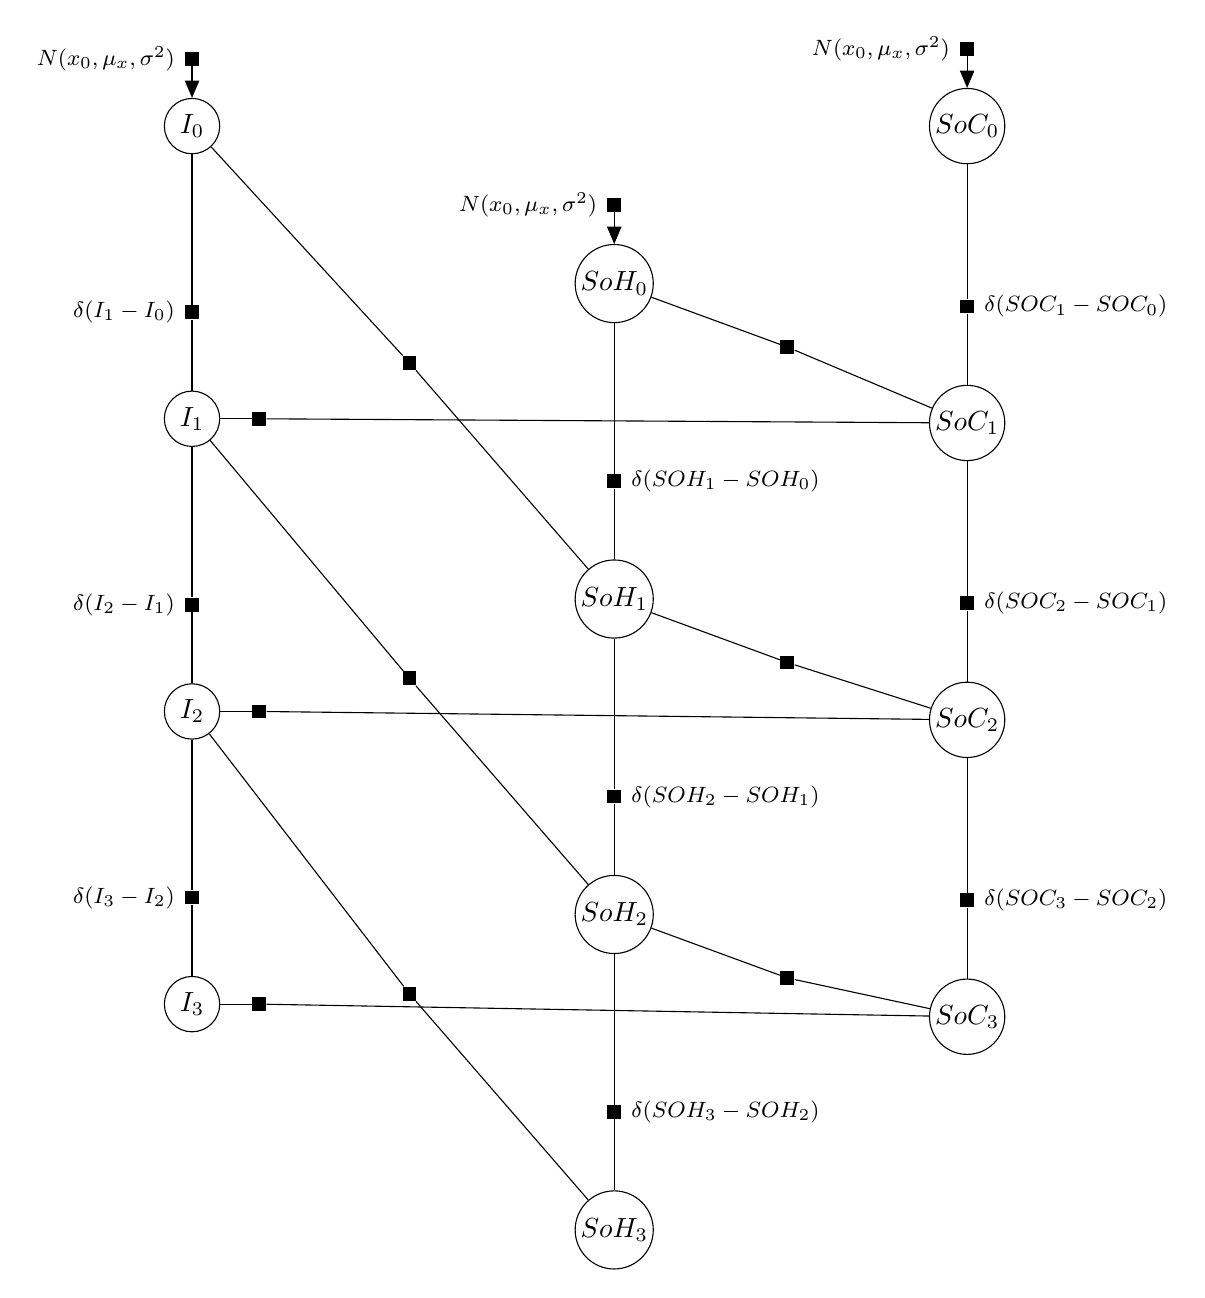
\begin{tikzpicture}
  % Nodes
  \node[latent] (I0) {$I_0$};
  \node[latent, below=of I0, yshift=-2cm] (I1) {$I_1$};
  \node[latent, below=of I1, yshift=-2cm] (I2) {$I_2$};
  \node[latent, below=of I2, yshift=-2cm] (I3) {$I_3$};

  \node[latent, right=of I0, yshift=-2cm, xshift=3.5cm] (SOH0) {$SoH_0$};
  \node[latent, below=of SOH0, yshift=-2cm] (SOH1) {$SoH_1$};
  \node[latent, below=of SOH1, yshift=-2cm] (SOH2) {$SoH_2$};
  \node[latent, below=of SOH2, yshift=-2cm] (SOH3) {$SoH_3$};

  \node[latent, right=of I0, xshift=8cm] (SOC0) {$SoC_0$};
  \node[latent, below=of SOC0, yshift=-1.8cm] (SOC1) {$SoC_1$};
  \node[latent, below=of SOC1, yshift=-1.8cm] (SOC2) {$SoC_2$};
  \node[latent, below=of SOC2, yshift=-1.8cm] (SOC3) {$SoC_3$};

  % Factors
  \factor[above=of I0] {f1} {left:$N(x_0, \mu_{x}, \sigma^2)$} {} {I0};
  \factor[above=of SOC0] {f2} {left:$N(x_0, \mu_{x}, \sigma^2)$} {} {SOC0};
  \factor[above=of SOH0] {f3} {left:$N(x_0, \mu_{x}, \sigma^2)$} {} {SOH0};

  
  \factor[above=of I1, yshift=0.5cm] {f4} {left:$\delta(I_1 - I_0)$} {I0,I1} {};
  \factor[above=of I2, yshift=0.5cm] {f5} {left:$\delta(I_2 - I_1)$} {I1,I2} {};
  \factor[above=of I3, yshift=0.5cm] {f6} {left:$\delta(I_3 - I_2)$} {I2,I3} {};

  \factor[above=of SOC1, yshift=0.5cm] {f7} {right:$\delta(SOC_1 - SOC_0)$} {SOC0,SOC1} {};
  \factor[above=of SOC2, yshift=0.5cm] {f8} {right:$\delta(SOC_2 - SOC_1)$} {SOC1,SOC2} {};
  \factor[above=of SOC3, yshift=0.5cm] {f9} {right:$\delta(SOC_3 - SOC_2)$} {SOC2,SOC3} {};

  \factor[above=of SOH1, yshift=0.5cm] {f7} {right:$\delta(SOH_1 - SOH_0)$} {SOH0,SOH1} {};
  \factor[above=of SOH2, yshift=0.5cm] {f8} {right:$\delta(SOH_2 - SOH_1)$} {SOH1,SOH2} {};
  \factor[above=of SOH3, yshift=0.5cm] {f9} {right:$\delta(SOH_3 - SOH_2)$} {SOH2,SOH3} {};

  \factor[above=of SOH1, yshift=2cm, xshift=-2.6cm] {f10} {} {I0,SOH1} {};
  \factor[above=of SOH2, yshift=2cm, xshift=-2.6cm] {f11} {} {I1,SOH2} {};
  \factor[above=of SOH3, yshift=2cm, xshift=-2.6cm] {f12} {} {I2,SOH3} {};

  \factor[right=of I1] {f13} {} {I1,SOC1} {};
  \factor[right=of I2] {f14} {} {I2,SOC2} {};
  \factor[right=of I3] {f15} {} {I3,SOC3} {};

  \factor[right=of SOH1, yshift=3.2cm, xshift=1.2cm] {f16} {} {SOH0,SOC1} {};
  \factor[right=of SOH2, yshift=3.2cm, xshift=1.2cm] {f17} {} {SOH1,SOC2} {};
  \factor[right=of SOH3, yshift=3.2cm, xshift=1.2cm] {f18} {} {SOH2,SOC3} {};
  

\end{tikzpicture}

\end{document}